\subsection{Windows}

Windows deli proces posodabljanja sistema na 4 dele: iskanje, prenos, namestitev in potrditev \cite{windows-update}.
Postopek namestitve posodobitev opravlja t.i. orkestrator (ang. \emph{orchestrator}).
Le-ta v primeru avtomatskih posodobitev čas iskanja izbere naključno, saj to zmanjša obremenitev na strežnikih s
posodobitvami.

V nasprotju z nekaterimi distribucijami Linux, Windows ponuja le kumulativne posodobitve, kar pomeni da se mora ob vsaki
posodobitvi prenesti celotna vsebina, ne le razlike od zadnje posodobitve - t.i. \emph{delta posodobitve}.

Zaradi velikosti posodobitev Windows za prenos uporablja diferencialno kompresijo
(ang. \emph{forward and reverse differentials}) \cite{windows-update-compression}, ki omogoča zmanjšanje velikosti
tudi do 40\% v primerjavi z nekompresiranimi datotekami \cite{windows-update-compression-2}.

\subsubsection{Iskanje posodobitev}

Orkestrator išče samo posodobitve, ki so bile dodane po zadnjem času iskanja, kar omogoči hitro in učinkovito najdenje.
Prav tako pred prenosom preveri vsa administratorska pravila glede posodobitev, npr. katere vrste posodobitev
naj se opravijo.

Windows deli posodobitve na več storitev, vsako zadolženo za svoj del operacijskega sistema.
Primeri storitev so \emph{Windows Update}, \emph{Microsoft Update}, \emph{Store}, \emph{Unspecified} in druge.

\begin{figure}[H]
    \centering
    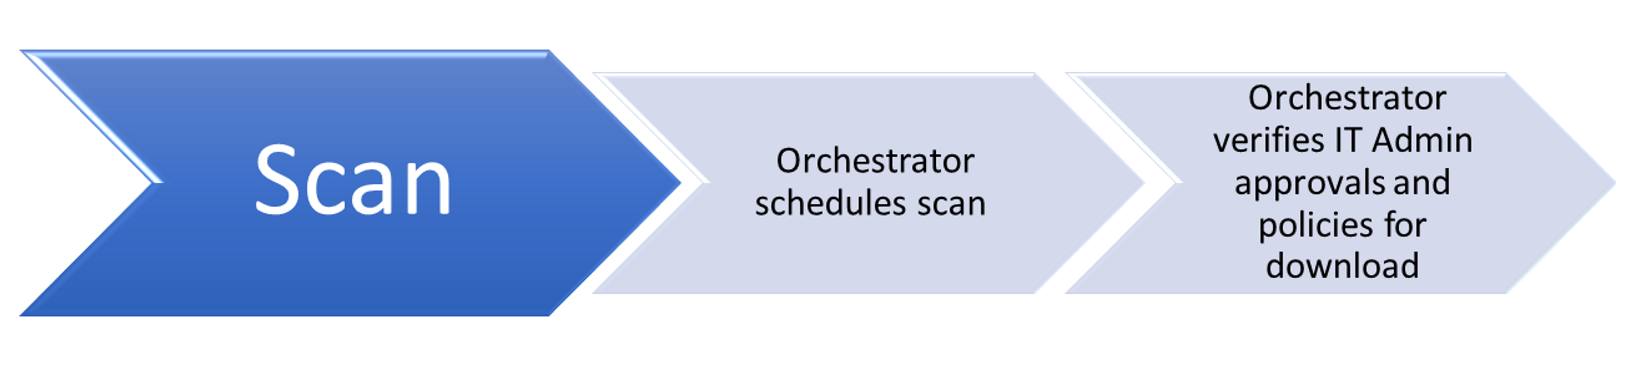
\includegraphics[width=0.7\textwidth]{windows-update-scan.png}
    \caption{Iskanje posodobitev na Windows \cite{windows-update}}
\end{figure}

\subsubsection{Prenos posodobitev}

Po izbiri posodobitev se začne njihov prenos. Le-ta se zgodi v ozadju in za preprečevanje zasičenosti omrežja
uporablja \emph{Delivery Optimization} (sl. optimizacijo prenosa), ki med drugim omogoča prenos posodobitev iz
drugih naprav Windows v omrežju.

\begin{figure}[H]
    \centering
    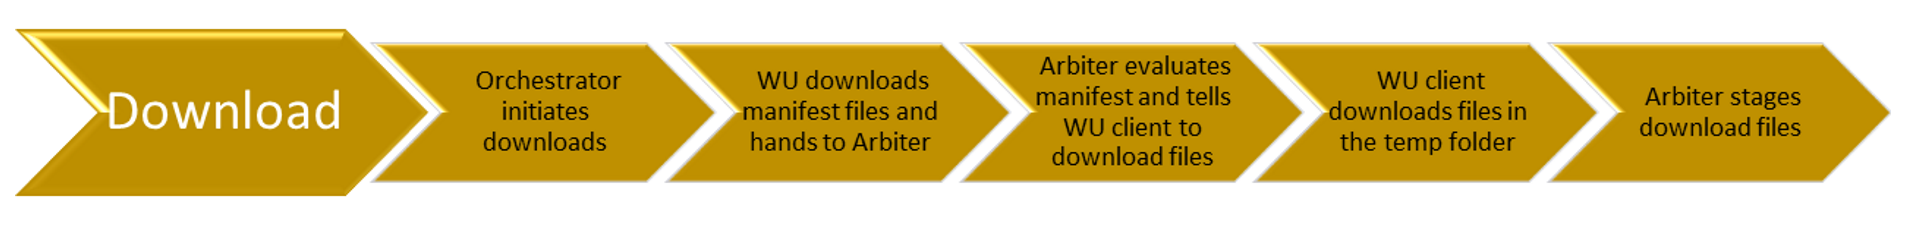
\includegraphics[width=1\textwidth]{windows-update-download.png}
    \caption{Prenos posodobitev na Windows \cite{windows-update}}
\end{figure}

\subsubsection{Namestitev posodobitev}

Del prenosa posodobitev vključuje metapodatke in t.i. \emph{Arbiter}, ki prebere konfiguracijo naprave in jo primerja
z metapodatki posodobitve, da ustvari seznam dejanj (ang. \emph{action list}).
Le-ta opisuje vse datoteke, ki so potrebne za namestitev posodobitve in dejanja, ki jih mora z njimi opraviti
namestitveni program.
Seznam dejanj je skupaj z vsebino posodobitve podan namestitvenemu programu, ki izvede namestitev.

\begin{figure}[H]
    \centering
    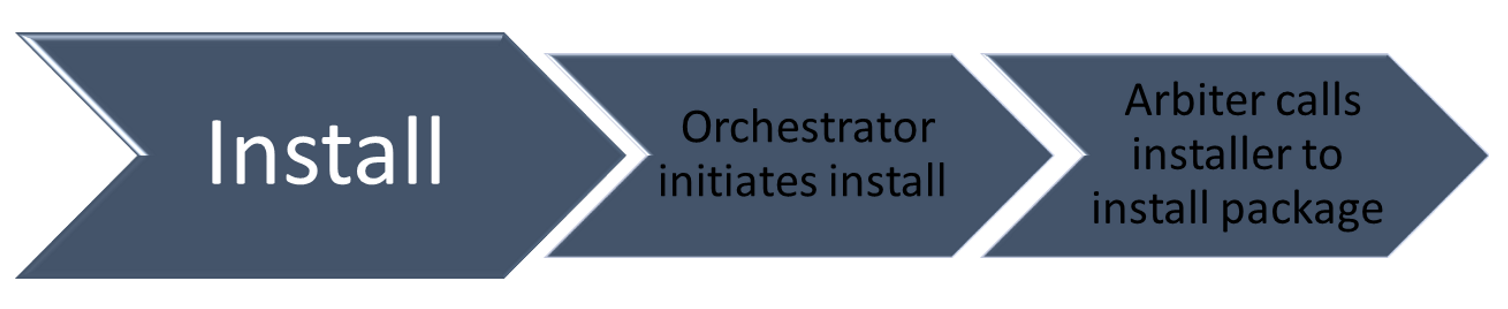
\includegraphics[width=0.7\textwidth]{windows-update-install.png}
    \caption{Namestitev posodobitev na Windows \cite{windows-update}}
\end{figure}

\subsubsection{Potrditev posodobitev}

Orkestrator kot zadnji korak v postopku nameščanja posodobitev v primeru avtomatskih posodobitev poskuša ponovno
zagnati napravo, saj je lahko le-ta nepopolno posodobljena dokler ni ponovno zagnana.

\begin{figure}[H]
    \centering
    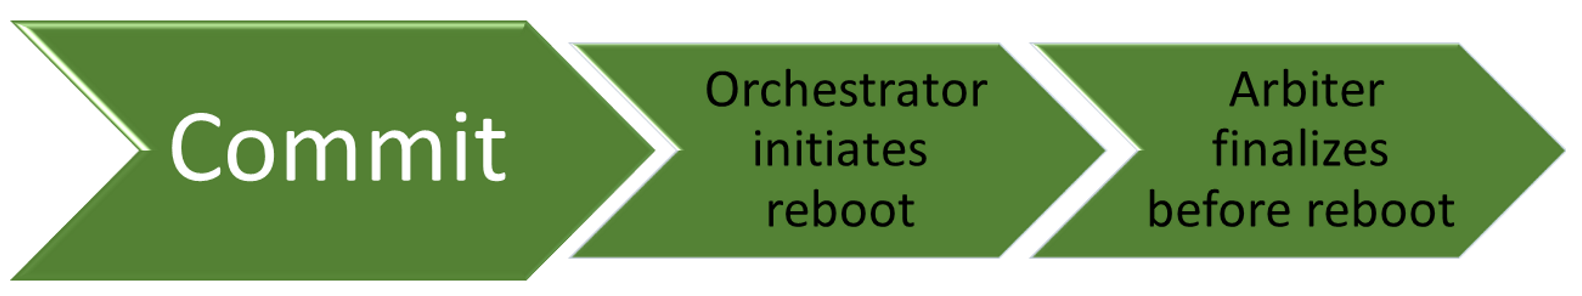
\includegraphics[width=0.7\textwidth]{windows-update-commit.png}
    \caption{Potrditev posodobitev na Windows \cite{windows-update}}
\end{figure}